\renewcommand{\theequation}{\theenumi}
\renewcommand{\thefigure}{\theenumi}
\renewcommand{\thetable}{\theenumi}
\begin{enumerate}[label=\thesection.\arabic*.,ref=\thesection.\theenumi]
\numberwithin{equation}{enumi}
\numberwithin{figure}{enumi}
\numberwithin{table}{enumi}


%
\item X and Y are independent random variables each having the density
\begin{align}
    f(t) = \displaystyle\frac{1}{\pi} \frac{1}{1+{t}^2} -\infty < t < +\infty
\end{align}
Then the density function of $\displaystyle\frac{X+Y}{3}$ for \\$-\infty <$ t $< +\infty$ is\bigskip
    \begin{enumerate}\itemsep0.5cm
        \item $\displaystyle\frac{6}{\pi} \frac{1}{4+9{t}^2}$
        \item $\displaystyle\frac{6}{\pi} \frac{1}{9+4{t}^2}$
        \item $\displaystyle\frac{3}{\pi} \frac{1}{1+9{t}^2}$
        \item $\displaystyle\frac{3}{\pi} \frac{1}{9+{t}^2}$
    \end{enumerate}

%
\solution
Let us consider the random variables X and Y.
    The Characteristic function of the probability density $f(t)$ is
    \begin{align}
        g(w) =\hspace{0.2cm} & \int_{-\infty}^{\infty}  f(t) {e}^{iwt} dt                                         \\[0.2cm]
        =\hspace{0.2cm}      & \int_{-\infty}^{\infty}  \displaystyle\frac{1}{\pi} \frac{1}{1+{t}^2} {e}^{iwt} dt \\[0.2cm]
        =\hspace{0.2cm}      & e^{-\abs{w}}\hspace{0.2cm}, -\infty<w<\infty
    \end{align}
    The product of the Characteristic function of \\probability density of X and Y is
    \begin{align}
        h(w) = g_1(w) \times g_2(w) = {e}^{-2\abs{w}}
    \end{align}
    To get the probability density of X+Y, we find the inverse characteristic function of h(w). But since there is a one to one correspondence between a function and its fourier transform and
$h(w) = g(2w)$
    \begin{align}
        F_{X+Y}(t) =\hspace{0.2cm} & \frac{1}{2}f\brak{\frac{t}{2}}                                        \\[0.2cm]
        =\hspace{0.2cm}            & \frac{1}{2\pi} \frac{4}{4+{t}^2} \hspace{0.2cm},-\infty<t<\infty
    \end{align}
    We know that if a random variable M has a\\probability density $f_M(x)$, then the probability \\density of random variable kM is
    \begin{align}
        f_{kM}\brak{x} = \frac{1}{\abs{k}} f_M\brak{\frac{x}{\abs{k}}}
    \end{align}
    Probability density of $Z = \displaystyle\frac{X+Y}{3}$ given $F_{X+Y}(t)$ is
\begin{align}
    F_{Z}(t) = & 3\times \displaystyle f_{X+Y}(3t) \\
    =          & \frac{6}{\pi} \frac{1}{4+9{t}^2}
\end{align}

\item Suppose X and Y are independent and identically distributed random variables and let $Z = X + Y$. Then the distribution of $Z$ is in the same family as that of $X$ and $Y$ if X is
\begin{table}[h]
\setlength{\tabcolsep}{30pt}
    \begin{tabular}{ll}
         1) Normal  & 2) Exponential  \\
         3) Uniform & 4) Binomial
    \end{tabular}
\end{table}
%
\solution


\begin{enumerate}[label = \arabic*)]
    \item Let X and Y be independent and identically distributed normal random variables. Then the characteristic function of X and Y is given by
    \begin{equation}
        \Phi_X(\omega) = e^{j\eta\omega - \sigma^2\omega^2/2}
    \end{equation}
    The characteristic function of Z is given by
    \begin{align}
        \Phi_Z(\omega) &= \Phi_X^2(\omega)\\
                       &= e^{2j\eta\omega - \sigma^2\omega^2}
    \end{align}
    Thus Z is a normal random variable with parameters $2\eta$ and $2\sigma^2$. Thus option (1) is correct.
    \item Let X and Y be independent and identically distributed exponential random variables. Then the characteristic function of X and Y is given by
    \begin{equation}
        \Phi_X(\omega) = \dfrac{\lambda}{1-j\omega}
    \end{equation}
    The characteristic function of Z is given by
    \begin{align}
        \Phi_Z(\omega) &= \Phi_X^2(\omega)\\
                       &= \dfrac{\lambda^2}{(1-j\omega)^2}
    \end{align}
    Thus Z is not an exponential random variable. Therefore option (2) is wrong.
    \item Let X and Y be independent and identically distributed uniform random variables such that X, Y $\sim$ U(a,b). Then the characteristic function of X and Y is given by
    \begin{equation}
        \Phi_X(\omega) = \dfrac{e^{jb\omega} - e^{ja\omega}}{j\omega(b-a)}
    \end{equation}
    The characteristic function of Z is given by
    \begin{align}
        \Phi_Z(\omega) &= \Phi_X^2(\omega)\\
                       &= -\dfrac{(e^{jb\omega} - e^{ja\omega})^2}{\omega^2(b-a)^2}
    \end{align}
    Thus Z is not a uniform random variable. Thus option (3) is wrong.
    \item Let X and Y be independent and identically distributed binomial random variables. Then the characteristic function of X and Y is given by
    \begin{equation}
        \Phi_X(\omega) = (pe^{j\omega}+q)^n
    \end{equation}
    The characteristic function of Z is given by
    \begin{align}
        \Phi_Z(\omega) &= \Phi_X^2(\omega)\\
                       &= (pe^{j\omega}+q)^{2n}
    \end{align}
    Thus Z is a binomial random variable with parameter 2n. Thus option (4) is correct.
\end{enumerate}
The following figures show the experimental distributions for Z in each case. The simulation length was kept one million.
\begin{figure}[!ht]
\centering
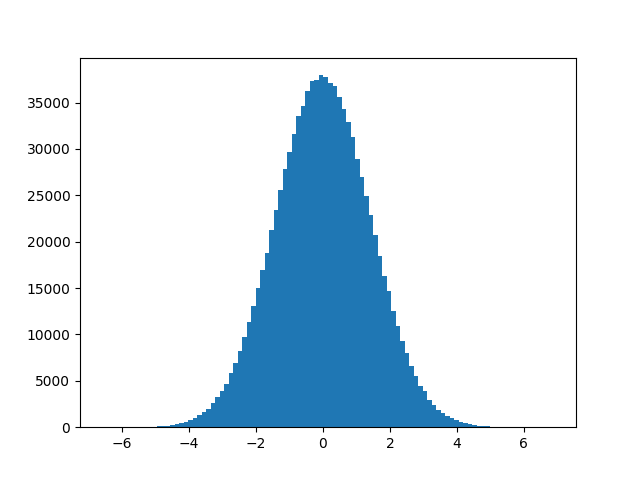
\includegraphics[width=\columnwidth]{solutions/2016/june/107/figures/norm.png}
\caption{Z when X is standard normal}
\label{june2016-107:fig:normal}
\end{figure}
\begin{figure}[!ht]
\centering
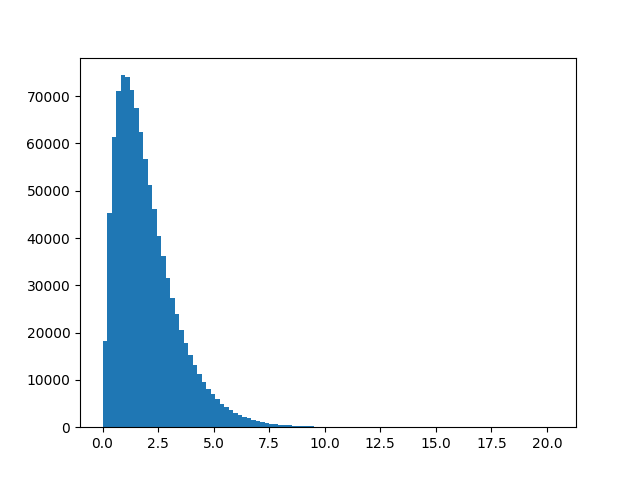
\includegraphics[width=\columnwidth]{solutions/2016/june/107/figures/expon.png}
\caption{Z when X is exponential with $\lambda = 1$}
\label{june2016-107:fig:exponential}
\end{figure}
\begin{figure}[!ht]
\centering
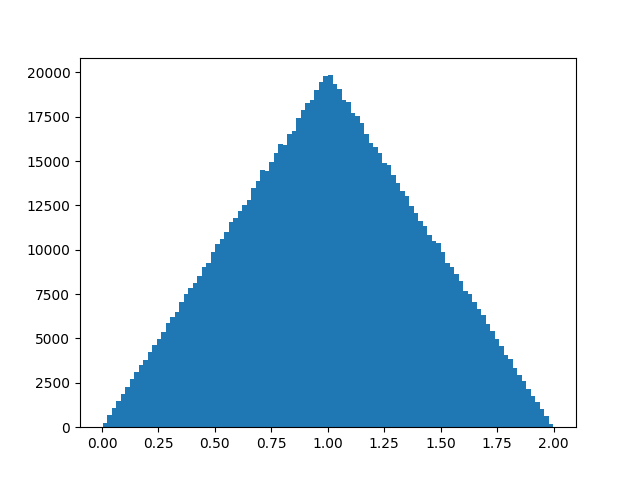
\includegraphics[width=\columnwidth]{solutions/2016/june/107/figures/uniform.png}
\caption{Z when X $\sim$ U(0,1)}
\label{june2016-107:fig:uniform}
\end{figure}
\begin{figure}[!ht]
\centering
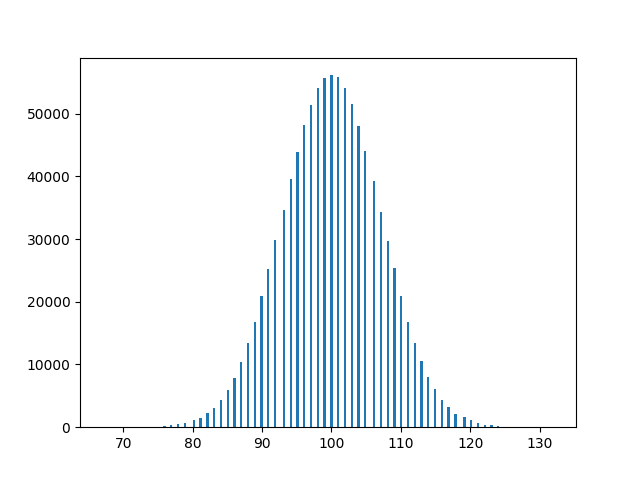
\includegraphics[width=\columnwidth]{solutions/2016/june/107/figures/binom.png}
\caption{Z when X $\sim$ B(100,0.5)}
\label{june2016-107:fig:binomial}
\end{figure}


\item  $N,A_1,A_2\cdots$ are independent real valued random variables such that 
    \begin{align}
        \pr{N=k}=(1-p)p^k,k=0,1,2,3\cdots
    \end{align}
    where $0<p<1$ and $\{A_i:i=1,2,\cdots\}$ is a sequence of independent and identically distributed bounded random variables. Let 
    \begin{align}
        X(w) = 
        \begin{cases}
        0  & \text{if } N(w)=0\\
        \sum_{j=1}^{k} A_j & \text{if } N(w)=k,k=1,2,3\cdots 
        \end{cases}
    \end{align}
    Which of the following are necessarily correct?\\
    \begin{enumerate}
        \item $X$ is a bounded random variable. 
        \item Moment generating function $m_X$ of $X$ is
        \begin{align}
            m_X(t)=\dfrac{1-p}{1-pm_A(t)}, t\in \mathbb{R},
        \end{align}
        where $m_A$ is moment generating function of $A_1$.
        \item Characteristic function $\varphi_X$ of $X$ is
        \begin{align}
            \varphi_X(t)=\dfrac{1-p}{1-p\varphi_A(t)},t\in \mathbb{R},
        \end{align}
        where $\varphi_A$ is the characteristic function of $A_1$.
        \item $X$ is symmetric about 0.
    \end{enumerate}

\end{enumerate}